
\renewcommand{\EntradaBibtex}{IdentificadorGeneroEspectrogramas_SistemasInteligentes_UPV_2024}

\begin{frame}{\citetitle{\EntradaBibtex}$^*$ (1)}
\begin{block}{Motivación} 
A partir de un audio personal, es posible determinar el género (biológico) de dicha persona
\begin{itemize}
\item Se grabaron audios de ambos generos
\item Se utilizó una librería para obtener su espectrograma
\item Se entrenó un modelo para clasificar imágenes de espectrograma obtenidos del audio grabado mediante la interfaz
\item Se creó una interfaz de usuario que vincula el grabador de sonidos del sistema con el modelo previamente entrenado
\end{itemize}
\end{block} 
\footfullcite*{\EntradaBibtex}
\end{frame}


\begin{frame}{\citetitle{\EntradaBibtex} (2)}
%\begin{block}{Pantallas Principales} 

%\begin{columns}
% Column 1
%\column{.1\linewidth}
%\begin{center}
%\includegraphics[width=0.85\linewidth]{2024_DetectorMotos/figs/resultados1.png}
%\includegraphics[width=0.85\linewidth]{2024_DetectorMotos/figs/resultados2.png}
%\end{center}
%\column{.9\linewidth}
\begin{center}
	\begin{tabular}{ccc} \hline
		Genero & Total de Pruebas & Aciertos \\
\hline
		Masculino & 29 & 23 (79\%) \\
		Femenito  & 23 & 19 (82\%)\\
		Total     & 52 & 42 (80\%)\\
\hline
	\end{tabular}
\end{center}

\begin{center}

	\begin{tabular}{cccc}
		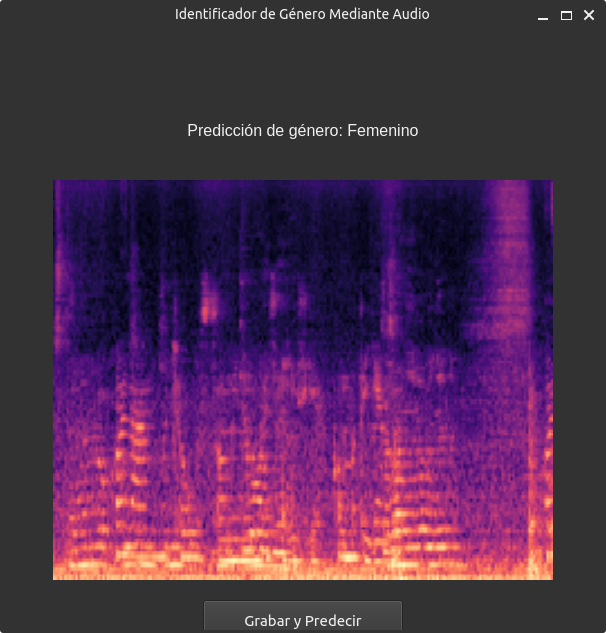
\includegraphics[width=0.20\linewidth]{2024_IdentificadorGeneroEspectrograma/figs/esp1.png} &
		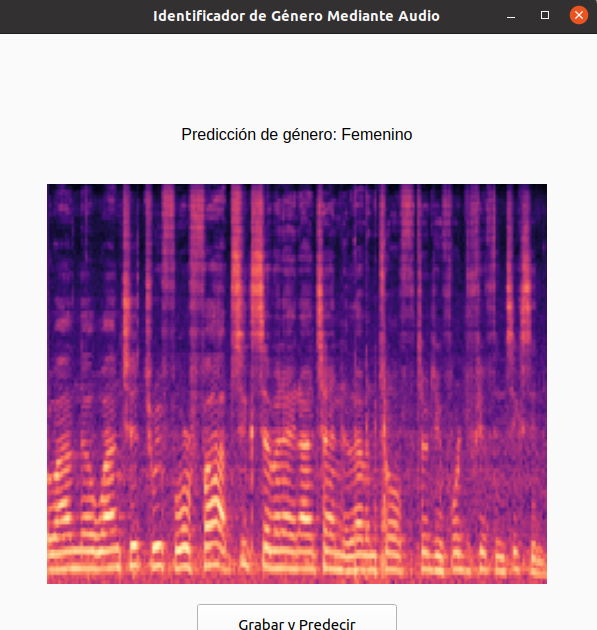
\includegraphics[width=0.20\linewidth]{2024_IdentificadorGeneroEspectrograma/figs/esp3.png} &
		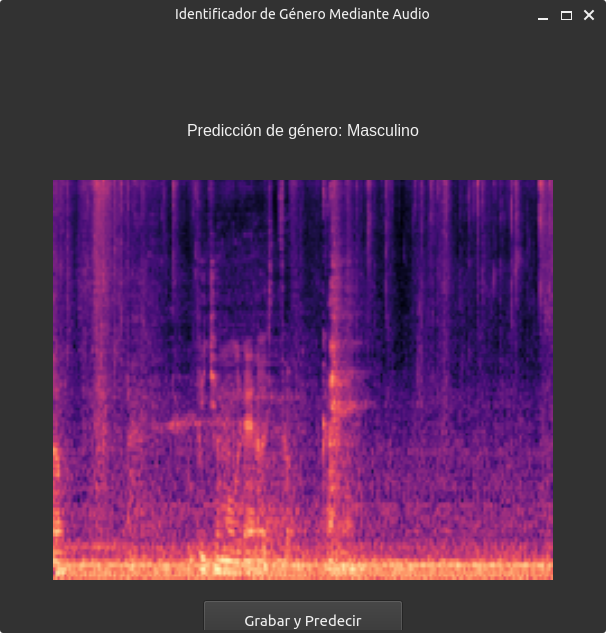
\includegraphics[width=0.20\linewidth]{2024_IdentificadorGeneroEspectrograma/figs/esp2.png} &
		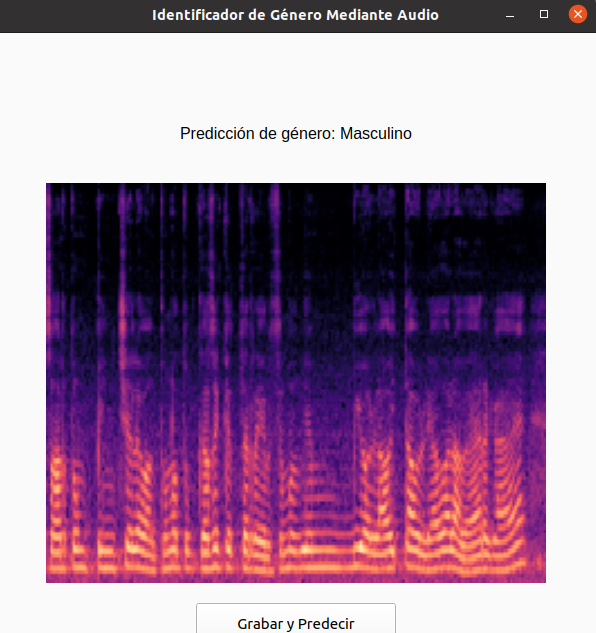
\includegraphics[width=0.20\linewidth]{2024_IdentificadorGeneroEspectrograma/figs/esp4.png} \\
	\end{tabular}
\end{center}

%\end{columns}
\end{frame}

